\documentclass[border=1pt, 12pt, tikz]{standalone}

\newcommand\wideOne{3cm}
\newcommand\wideTwo{4cm}
\newcommand\wideThree{2.7cm}
\newcommand\wideFour{3cm}
\newcommand\distOne{2cm}
\newcommand\distTwo{1cm}

\begin{document}
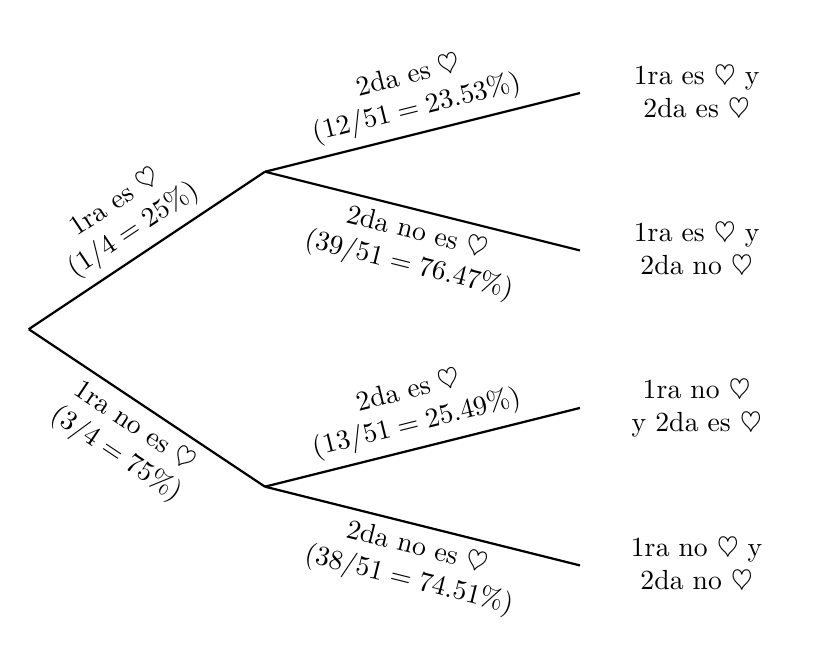
\begin{tikzpicture}[scale=1]

% 1ra level
\draw[thick]%
   (0,0) 
   -- node[above, sloped, align=center]
      {\textcolor{black}{1ra es $\heartsuit$}\\$(1/4=25\%)$} 
   (\wideOne,\distOne);
\draw[thick] 
   (0,0) 
   -- node[below, sloped, align=center]
      {\textcolor{black}{1ra no es $\heartsuit$}\\($3/4=75\%$)} 
   (\wideOne,-\distOne);

% 2da, 3rd and 4th Level
\draw[thick] 
   (\wideOne,\distOne)
   -- node[above, align=center, sloped]
      {2da es $\heartsuit$\\$(12/51=23.53\%)$}
   ++ (\wideTwo,\distTwo) 
      node[right, align=center, text width=\wideThree]
      {1ra es $\heartsuit$ y\\2da es $\heartsuit$}
   ; 
\draw[thick] 
   (\wideOne,\distOne) 
   -- node[below, align=center, sloped]
      {2da no es $\heartsuit$\\($39/51=76.47\%$)}
   ++ (\wideTwo,-\distTwo) 
      node[right, align=center, text width=\wideThree]
      {1ra es $\heartsuit$ y 2da no $\heartsuit$}
   ;
\draw[thick] 
   (\wideOne,-\distOne) 
   -- node[above, align=center, sloped]
      {2da es $\heartsuit$\\$(13/51=25.49\%)$}
   ++ (\wideTwo,\distTwo) 
      node[right, align=center, text width=\wideThree]
      {\textcolor{black}{1ra no $\heartsuit$ y 2da es $\heartsuit$}}
   ;  
\draw[thick] 
   (\wideOne,-\distOne)
   -- node[below, align=center, sloped]
      {2da no es $\heartsuit$\\($38/51=74.51\%$)}
   ++ (\wideTwo,-\distTwo) 
      node[right, align=center, text width=\wideThree]
      {1ra no $\heartsuit$ y 2da no $\heartsuit$}
   ; 
\end{tikzpicture}
\end{document}

